\chapter{Dokumentenmanagement}
Das CMS System ist mit einem Dokumentenmanagementsystem gekoppelt. 
Klickt man auf das Symbol zum Einf�gen eines Links oder eines Bildes 
erh�lt man neben dem Eingabefeld f�r die URL ein kleines Symbol (1).
\begin{figure}
	\begin{center}
    \begin{picture}(56,45)
			\put(0,0){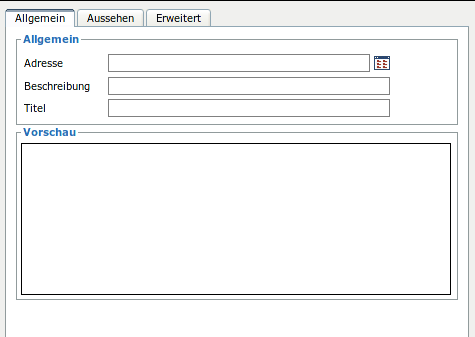
\includegraphics[height=40mm, width=56mm]{dms_erweitert_icon.png}}
			\markier{1}{52}{39}{-1}{-1}
		\end{picture}
    \caption{Dokumentenauswahl}
		\label{Dokumentenauswahl}
  \end{center}
\end{figure}

Hier gelangt man in das Dokumentenmanagementsystem.
Dokumente k�nnen hier hochgeladen und Kategorien zugeordnet werden. 
Mit einem klick auf den Namen wird die Datei ausgew�hlt und in den Editor eingef�gt.
\section{Hochladen von Dateien}
- Kategorie ausw�hlen\\
- "Datei hochladen" klicken\\
- im unteren Teil wird ein Formular angezeigt. Hier kann die Datei gesucht und
hochgeladen werden. \\
\section{Neue Version hochladen}
- Datei suchen\\
- Erweitert->Neue Version hochladen\\
- Datei ausw�hlen und hochladen\\

\section{Kategorien}
Damit die Dokumente nicht bunt durcheinandergemisch sind, k�nnen diese in
Kategorien zusammengefasst werden. Ein Dokument kann immer nur einer Kategorie
zugewiesen sein.

\section{Zugriffsrechte}
Der Zugriff auf Dokumente wird �ber die Kategorien gesteuert.\\
Zu jeder Kategorie k�nnen Gruppen zugeordnet werden. Die Mitglieder dieser Gruppe haben
dann Zugriff auf die Dokumente innerhalb dieser Kategorie. Die Rechte werden an die
darunterliegenden Kategorien vererbt.\\
Wenn keine Gruppenzuordnung f�r die Kategorie oder �bergeordneten Kategorien vorhanden ist, dann ist die Datei frei f�r alle zug�nglich.\\
\\
Eine Ausnahme stellen die Projektdokumente dar. Sobald ein Dokument zu einem Projekt zugeordnet ist, ist dieses Dokument nur noch von den Personen einsehbar, welche dem entsprechenden Projekt zugeordnet sind.\\
\\
F�r Administratoren kann die Berechtigung 'basis/dms' vergeben werden. Mit diesem Recht kann auf alle Dokumente zugegriffen werden.\\
\\
Gesperrte Kategorien werden im DMS System mit einem Schloss Symbol versehen.